\documentclass[a4paper,11pt]{book}
\usepackage{import}
\usepackage{preamb}

\makeindex

\begin{document}

\small
\begin{multicols}{3}

%\maketitle

\thispagestyle{empty}
\scriptsize
\newpage


\begin{subbox}{subbox}{}
\centering
\Large{\textbf{Network Science   \\ Cheatsheet}}
\end{subbox}

\begin{multibox}{2}
\begin{subbox}{subbox}{}
\centering

\includegraphics[width=0.8\textwidth]{pics/logo.png}
\end{subbox}
\begin{subbox}{subbox}{}
\centering
Made by \\
\large{
Remy Cazabet
}
\end{subbox}
\end{multibox}
% \section{Blocks and Community structure}


\begin{subbox}{subbox}{}
\centering
\Large{\textbf{Machine Learning on Graphs}}
\end{subbox}

\begin{subbox}{subbox}{}
This class is about Machine Learning on graphs \textbf{without} using graph embedding and Graph Convolutional Networks. For those techniques, see the next class.
\end{subbox}



\begin{textbox}{Machine Learning}
\textit{Machine learning(ML) involves computers discovering how they can perform tasks without being explicitly programmed to do so. It involves computers learning from data provided so that they carry out certain tasks}\footnote{\url{https://en.wikipedia.org/wiki/Machine_learning}}. It is a subset of \textbf{Artificial Intelligence}.

\end{textbox}




\begin{textbox}{Unsupervised ML}
In unsupervised learning, the machine is presented with the data, but without any examples. It should infer automatically the rules, the organization of the data.

A typical example of unsupervised ML is the \textbf{clustering} task. Community detection is a type of clustering on networks, that we have already discussed, so this class will rather focus on Supervised ML.
\end{textbox}


\begin{textbox}{Supervised ML}
\textit{Supervised learning is the machine learning task of learning a function that maps an input to an output based on example input-output pairs.}

After seeing enough examples structured as: input $\rightarrow$ output, the machine generalizes a knowledge such as for any (unseen) input, it will predict an output.

Examples: Given properties of an apartment, predict its energy consumption or price. Given a picture, recognize objects in it. Given a patient profile, predict effect of a drug. etc.

\end{textbox}









\begin{textbox}{Link Prediction}
Link prediction is a typical machine learning task on networks.

Examples of applications are the prediction that an edge might appear in the future (e.g., in dynamic networks), the discovery of missing links in, existing in the studied system but absent from our graph model (e.g., missing synonyms in Wiktionary, unknown gene-disease interactions, etc.), or for recommendation: profile recommendation in social medias, content recommendation in online retailers or service providers (Netflix, Spotify, YouTube, etc.).

Link prediction can be based only on the network structure, or on a mixture of network structure and node properties.  
\end{textbox}



\begin{textbox}{Link Prediction: intuition}
How likely it is for an edge to appear between nodes can depend on:
\begin{itemize}
    \item Local factors: I'm more likely to connect with friends of my friends than with random nodes.
    \item Nodes properties/attributes: Nodes with high degrees are statistically more likely to bond than nodes with few edges. Age, political opinions, spatial proximity might be correlated with edge existence (assortativity, spatial networks, etc.)
    \item Meso-scale structure: Nodes belonging to the same (automatically discovered) communities might be more likely to connect, for instance.
\end{itemize}
\end{textbox}





\begin{textbox}{Link Prediction: Heuristics}
A fist approach to predict edges is not based on machine learning, but consists in defining  \textbf{heuristics}, based on the intuitions developed above: shared neighborhood, nodes degrees, meso-scale structure, etc.
\end{textbox}

\begin{textbox}{Heuristic: Common neighbors (CN)}
Hypothesis: the \textbf{number} of common neighbors is an indicator of the probability to connect. Based on the "friends of my friends are my friends", transitivity principle.

\[
CN(u,v)=|N(u)\cap N(v)|
\]

\end{textbox}

\begin{textbox}{Heuristic: Jaccard Coefficient (JC)}
Hypothesis: The \textbf{fraction} of common neighbors might be more relevant than the raw number of common neighbors.

\[
JC(u,v)=\frac{|N(u)\cap N(v)|}{|N(u)\cup N(v)|}
\]

\end{textbox}


\begin{textbox}{Heuristic: Hub Promoted (HP)}
Hypothesis: Considers the fraction of common neighbors for the node of lower degree. Can discover star-following relationships (10 of my friends follow a star, vs two stars have 10 followers in common).
%Hypothesis: the relation can be asymmetrical: if one of the nodes has a high fraction of its neighbors in common with the other, it might be likely to connect with it, even if the contrary is not true (e.g., all of my friends follow celebrity $x$, so I'm likely to follow $x$, even if $x$ has a large number of followers who are not my friend)
\[
HP(u,v)=\frac{|N(u)\cap N(v)|}{\min(|N(u)|,| N(v)|}
\]

Variant: Hub Depressed (HD)
\[
HD(u,v)=\frac{|N(u)\cap N(v)|}{\max(|N(u)|,| N(v)|}
\]
\end{textbox}



\begin{textbox}{Heuristic: Adamic Adar (AA)}
Hypothesis: all neighbors are not worth the same, neighbors with a small degree are more significant than hubs (e.g., you and me having two close friends in common is more significant than following the same two celebrities with millions of followers.)

\[
AA(u,v)=\sum_{w\in N(u)\cap N(v)} \frac{1}{\log (k_w)}
\]

\end{textbox}


\begin{textbox}{Heuristic: Resource Allocation (RA)}
Hypothesis: Similar to AA, but penalizes more higher degrees.

\[
RA(u,v)=\sum_{w\in N(u)\cap N(v)} \frac{1}{k_w}
\]

\end{textbox}



\begin{textbox}{Heuristic: Preferential Attachment (PA)}
Hypothesis: As known from the Configuration Model, nodes with higher degrees are more likely to be connected.

\[
PA(u,v)=k_u k_v
\]

Note that unlike previous ones, this heuristic gives non-zero scores to nodes at distances larger than 2.
\end{textbox}


\begin{textbox}{Heuristic: Other scores}
Several other scores based on similar ideas have been proposed in the literature\footcite{zhou2009predicting}(Sorenson Index, Salton Cosine Similarity, Leicht-Holme-Nerman, etc.)

Which heuristic is the most appropriate for link prediction has no straightforward answer. 


\end{textbox}



\begin{textbox}{Heuristic: Distances - Random Walk}
Another family of heuristics to assess node likelihood to connect consists in using their network distance as a proxy. Much as nodes which are close in geographical space tends to connect with higher probability, nodes located close in the topology of the network are usually more likely to connect. It can be seen as an extension of the principle of common neighbors to nodes at farther distances.

Methods to measure the distance between nodes can consist\footcite{lichtenwalter2010new} in using the shortest-path distance, the probability to reach a node from another on a random walk, or the number of paths of a chosen length $l$ between them.


\end{textbox}






\begin{textbox}{Heuristic: Community Structure}
The community structure detected by an algorithm can be used as a heuristic for link prediction. The exact way to rank pairs of nodes from more likely to less likely to be connected depends on the community detection algorithm used\footcite{ghasemian2019evaluating}:

For methods optimizing a global quality function, such as Modularity or Infomap Information compression, the \textit{score} between each pair of nodes is proportional to the gain (or loss) in the global score if this edge were added. For instance, with Modularity, adding edges inside communities will tend to increase the global score (edges considered likely), while edges between communities will decrease it (unlikely edges).

For methods based on Stochastic Block Models, the score associated to a node is directly yielded by the model: the block matrix can be interpreted as describing the probability of an edge to exist between any two nodes belonging to a particular pair of blocks. In degree-corrected SBM, edge probabilities depends both of their blocks and of their degrees.


\end{textbox}



\begin{textbox}{Heuristic: Spatial Networks}
If a spatial model (Gravity, Radiation, etc.) has been fit on a spatial graph, then the probability of any edge appearing is given by the model, much as for SBM. 

The logic is the same for any kind of node properties, although, if there is no natural notion of distance for these properties, it is more efficient to let the machine learning algorithm learn the best way to combine them.
\end{textbox}





\begin{textbox}{From Heuristics to supervised ML}
Heuristics can directly be used for link prediction, but, since they capture different types of properties (local/meso/global), using only one of them means missing the information brought by the others.

Supervised Machine Learning is the most efficient way to combine them: since we do not know \textit{a priori} how to combine them, and the optimal way to do so might depend on the network, we let the computer learn how to do it.


\end{textbox}






\begin{textbox}{Training for link prediction}
Training a ML algorithm requires to constitute a \textbf{training set}, i.e., a set of examples \textit{input}$\rightarrow$ \textit{output}. For link predictions, an example is composed of:
\begin{itemize}
    \item Input: Heuristics associated to the node pair
    \item Output: 1 or 0 (Respectively, an edge exists or not between those 2 nodes in the original graph.)
\end{itemize}

Since we want to predict edges that are \textit{not yet} on the network, we start by removing $t$ edges from the network, that will constitute \textbf{positive examples} for training. We sample $t$ other node pairs that are \textbf{not} connected by an edge in the original graph: they are \textbf{negative examples}. 

Our training set is therefore composed of a balanced (50\% negative, 50\% positive) set of $2t$ examples.  
\end{textbox}


\begin{textbox}{Training - Prediction}
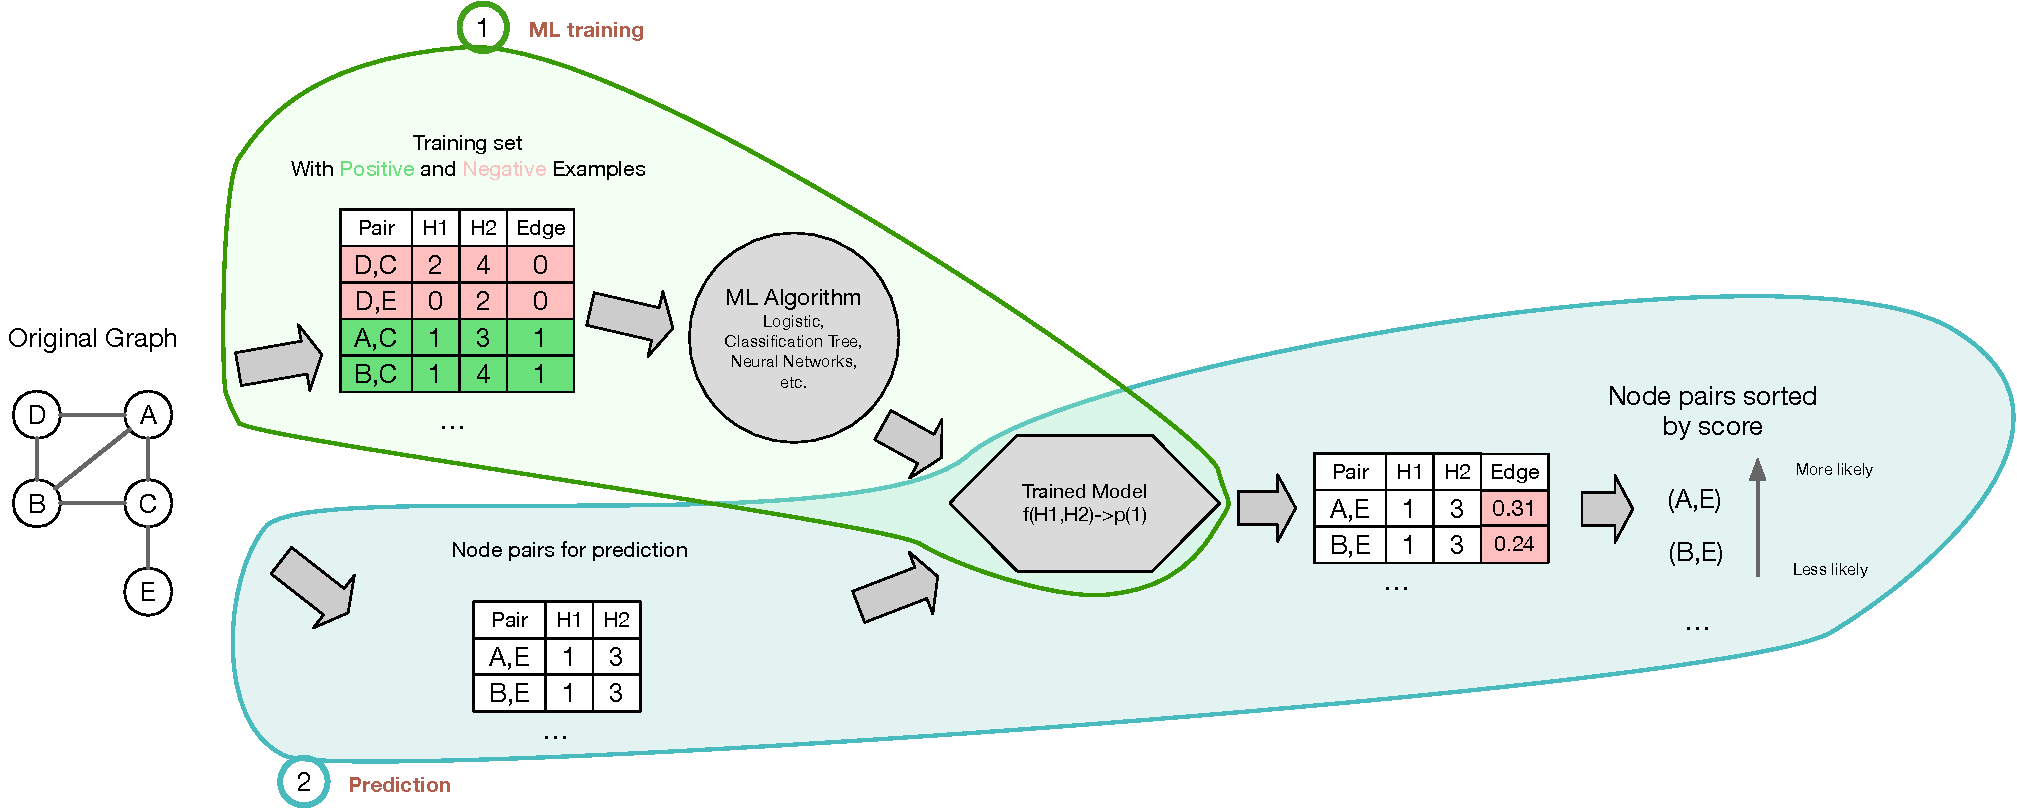
\includegraphics[width=\textwidth]{pics/train-predict.pdf}
\end{textbox}


\begin{textbox}{ML algorithm: Classifiers}
Supervised Machine Learning is usually split between methods that predict numerical values (\textbf{Regression}), and those who predict to which class an element belongs, among several choices (\textbf{Classification}). Link prediction is usually made with classification algorithms (Two classes: Edge or Not-Edge). 

A wide variety of such algorithms exist, from simple Linear Regressors to deep neural networks. Implementations and description of algorithms can be found, for instance, in the popular scikit-learn library\footnote{\url{https://scikit-learn.org/stable/supervised_learning.html}}. Good places to start are Logistic classifiers and Decision Trees.
\end{textbox}






\begin{textbox}{Classifier results}
A trained Classifier is a model which, presented a set of features, yields a probability to belong to a particular class. While in other applications, we consider the most likly class as the answer, in link prediction, most of the time, we are interested in the probability itself. 

We use this probability to \textbf{rank} pairs of nodes, from the most to the least likely of being connected by an edge.
\end{textbox}




\begin{textbox}{Evaluation in Machine Learning}
In the Machine Learning scientific field, the evaluation of the effectiveness of algorithms is a central question. The evaluation is usually done as follows: The original set of observations is split in 2, the \textbf{training set} and the \textbf{test set} (evaluation set). The model is trained on the training set, without access to the test set, and the performance of the trained model is evaluated on the test set.

\end{textbox}



\begin{textbox}{Evaluation in Link prediction}
Link prediction quality evaluation(testing) is a little special compared with non-graph quality evaluation, since we do not start with a set of observations, but a single observation of a graph. We cannot split the graph in training and test graphs, so we consider pairs of nodes as observations, although this introduces biases: the graph on which we train is not the same as the one used for testing: they have different number of edges, some nodes have different degrees, etc.

Note also that the original graph is split in 3: the training set (sample of node pairs), the test set (sample of node pairs) and the original graph without edges of the training and test sets, used to compute the features/heuristics. 
\end{textbox}

\begin{textbox}{Training - Evaluation}
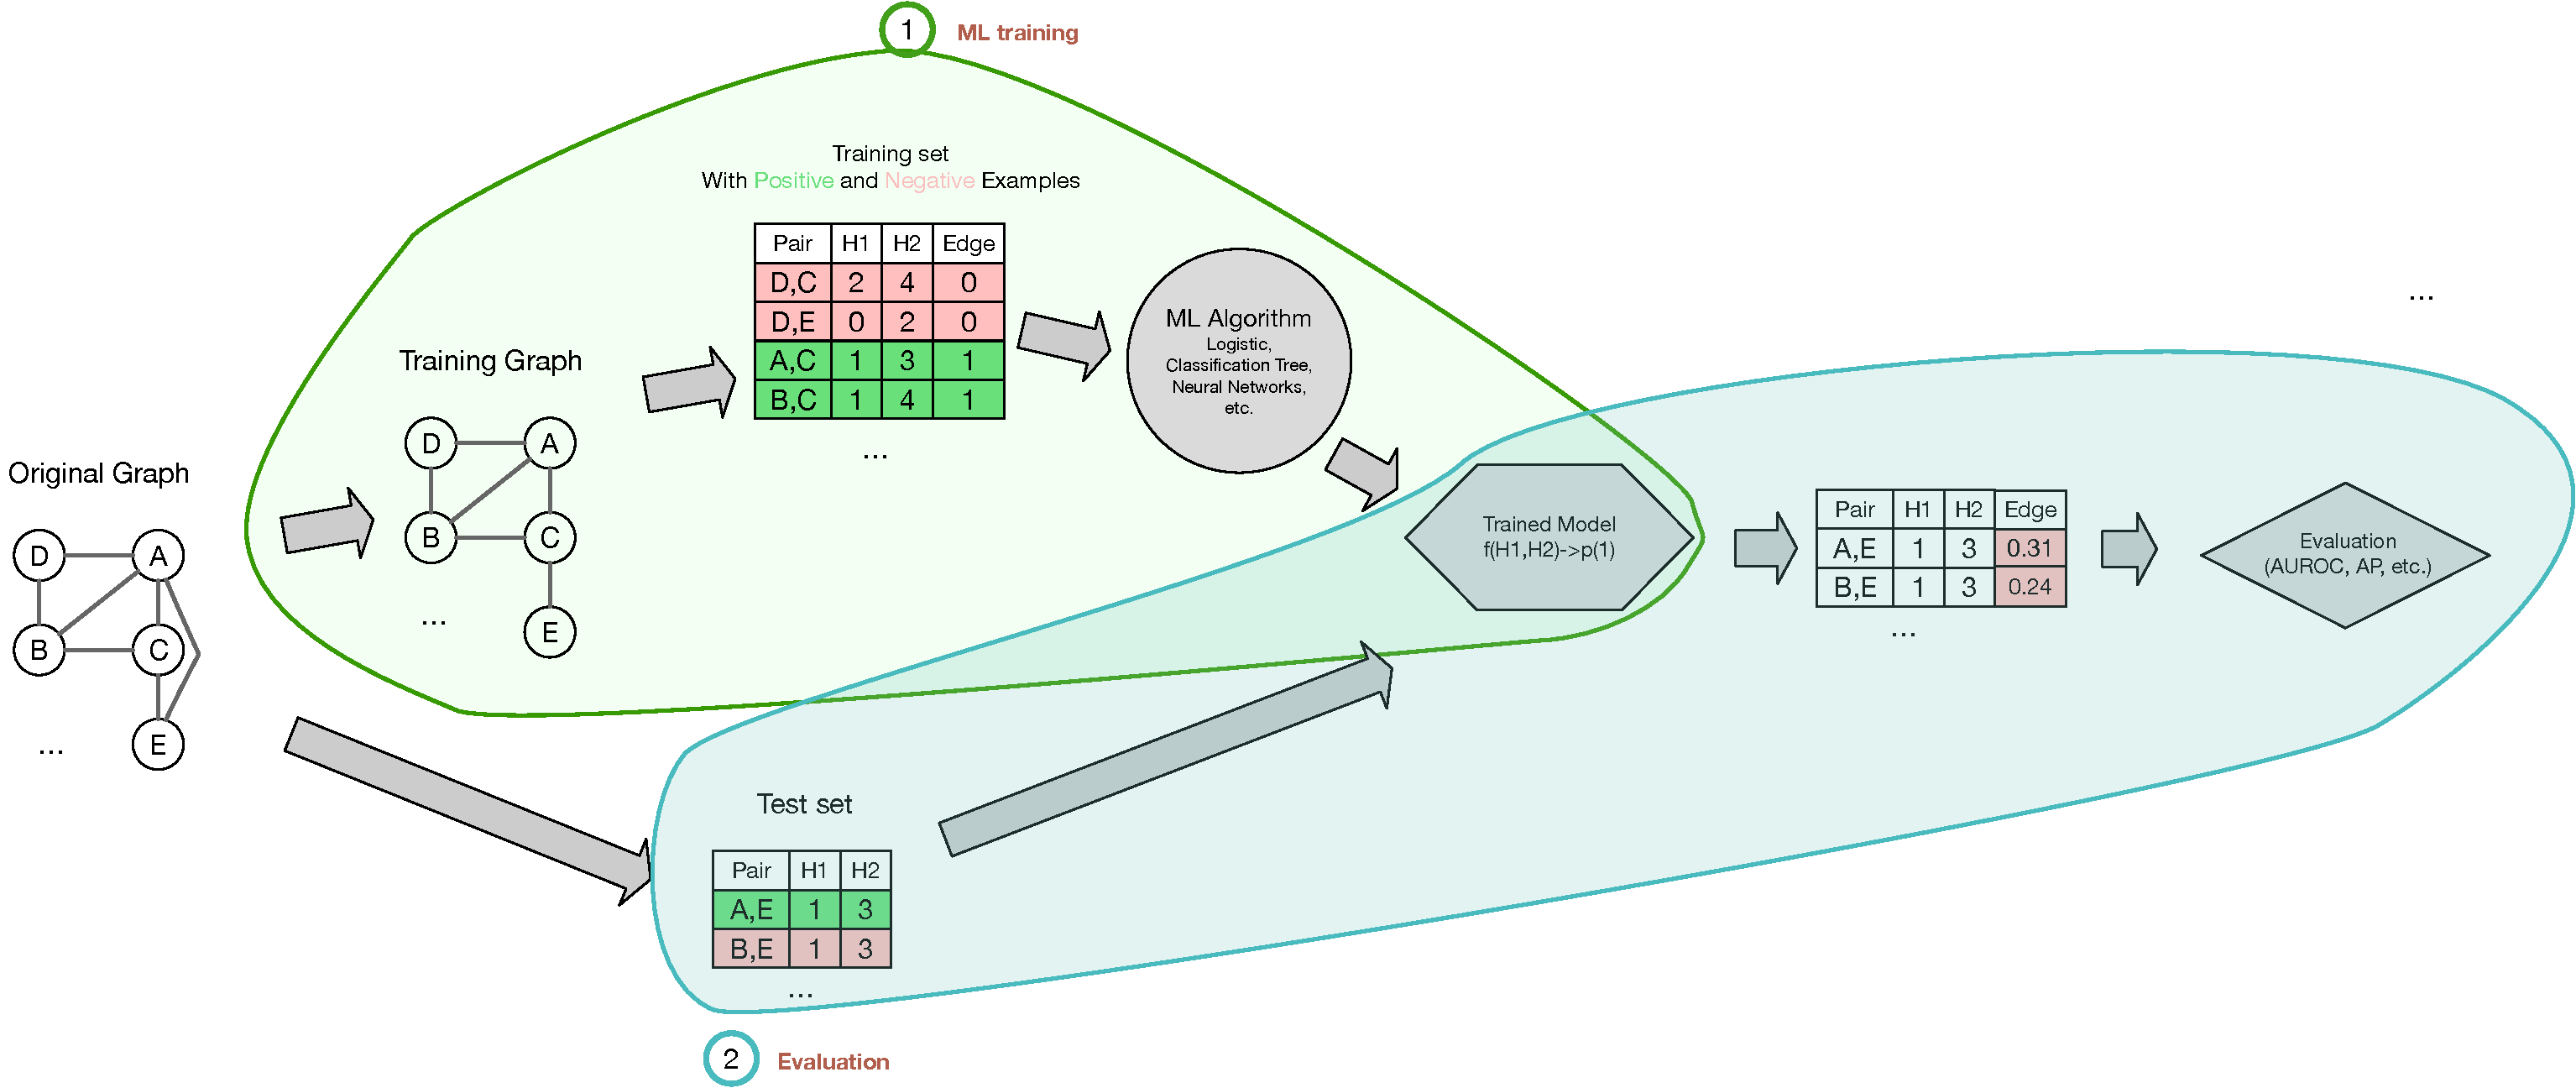
\includegraphics[width=\textwidth]{pics/train-test.pdf}
\end{textbox}

\begin{textbox}{Balanced training - Unbalanced test sets}
Training and test sets must be composed of positive and negatives examples, respectively node pairs between which we have to predict an edge or a non-edge.
For link prediction, the problem is that the set of all node pairs is usually extremely unbalanced. Networks are sparse, thus it is common in large graphs to have only one edge every 10,000 node pairs, for instance.

\begin{itemize}
    \item The balance of the training set can be chosen freely: What we care is to have a well-trained model, whatever the means. It is usually balanced because it is more efficient and convenient.
    \item The test set on the contrary must, in principle, respect the original balance between edges and non-edges: the method must be tested in real conditions, not on an artificially simplified problem. 
\end{itemize}

\end{textbox}




\begin{textbox}{Classification evaluation: Precision@k}
Precision@k is defined as the fraction of positive examples among the $k$ pairs of nodes of highest score according to the classifier.

The weakness of this approach is that the result depends on the chosen $k$. 
\end{textbox}




\begin{textbox}{Classification evaluation: Average precision}
Average precision, also known as Area Under the Precision/Recall Curve, is defined as the average Precision@k for all $k$.
\end{textbox}



\begin{textbox}{Classification evaluation: AUC/AUROC}
Area Under the Receiver Operating Characteristic Curve (\textbf{AUROC}), often simply abbreviated as \textbf{AUC} (Area Under the Curve), is defined as the area under the curve defined with False Positives on the horizontal axis and True Positives on the vertical axis. 
It has an intuitive probabilistic interpretation: the AUROC score corresponds to the probability, if we take two pairs of nodes at random, one a positive example and the other a negative one, that the positive example is ranked higher than the negative one. 

The score thus lies between 0 and 1, and a score of 0.5 corresponds to a random prediction.

The main advantage over previous scores is that in theory, its value does not depend on the balance of the test set.

AUC is currently the most used evaluation score, although some limitations have been raised\footcite{yang2015evaluating}.
\end{textbox}




\begin{textbox}{Machine Learning for nodes}
The other main application of ML on graphs is to predict some node properties, being numerical values (regression) or classes (classification).

Among applications, we can cite the filling of missing values (e.g., speed limits in a road network, categories of Wikipedia article, etc.), the prediction of unknown/hidden attributes (e.g., in marketing, knowing the gender, political opinion, age, salary, etc.), or the detection of particular nodes (spammers, bots, fake accounts, etc.)


\end{textbox}

\begin{textbox}{Non-network approaches}
If there are several properties on nodes, some of these properties can be used as input to predict another one as output. For instance individuals age, gender, and political opinions could be used to predict (efficiently or not) the revenue of these same individuals, if we can collect training examples. (Note: machine learning works based on correlation, not causation)
\end{textbox}


\begin{textbox}{Centrality as attributes}
A simple approach to improve the prediction consists in integrating some network properties computed on the node in the prediction. For instance, additionally to age, gender and opinions, one could integrate the degree, betweenness, closeness, clustering coefficient, etc. of a node in the prediction of its revenue. 
\end{textbox}


\begin{textbox}{Neighbors attributes as ego attributes}
Following the popular saying "Tell me who your friends are and I will tell you who you are", we can use the network to observe what are the most common features of the neighbors of a target node to predict its own features. For instance, the revenues of your neighbors in the graph might be useful to predict your own revenue. Furthermore, the most common political opinion, or the average age of the neighbors can also be a useful hint.

In practice, a simple way to do this consists\footcite{bhagat2011node} in computing, for each node feature, the average value of those features in the neighborhood of nodes. A simple ML model can then be used as if those properties were the nodes own properties.
\end{textbox}





\begin{textbox}{Random Walk attributes estimation}
A generalization of the previous approach consists in evaluating the distribution of attributes not only among the direct neighbors of the target nodes, but more generally among nodes that are close from it in the graph. A simple way to achieve this is to sample attributes using random walks. Several methods exist\footcite{bhagat2011node}, for instance for a numerical attribute, the estimated value $\tilde{y_u}[c]$ for attribute $c$ for node $u$ can be expressed as the average value encountered by a random walk of length $l$. More formally:
\[
\tilde{y_u}[c]= \sum_{v \in V}p_{uv}^l v[c]
\]

with $p_{ij}^l$ the probability to encounter node $v$ from node $u$ after a random walk of length $l$, and  $v[c]$ the value of label $c$ for node $v$
\end{textbox}




\begin{textbox}{Going Further}
Python Library: \url{scikit-learn}

Surveys: (\cite{lichtenwalter2010new}) (\cite{al2006link}) (\cite{lu2011link}) 

Model stacking: (\cite{ghasemian2020stacking})

Evaluation of link prediction: (\cite{yang2015evaluating})

Node Classification: (\cite{bhagat2011node})

Underfit and Overfit of community-based link prediction: (\cite{ghasemian2019evaluating})

Using Graphlets for machine learning: (\cite{rahman2016link}) 

Splitting train/test sets in networks: (\cite{deexperimental}

\end{textbox}







 \AtNextBibliography{\footnotesize}


\printbibliography[heading=subbibliography]


\end{multicols}



\end{document}


